\documentclass[11pt, a4paper]{article}
\usepackage[T1]{fontenc}
\usepackage[utf8]{inputenc}
\usepackage{lmodern}
\usepackage[margin=2cm, top=2.5cm, bottom=2.5cm, headheight=14pt]{geometry}
\usepackage{amsmath}
\usepackage{amssymb}
\usepackage[table]{xcolor}
\usepackage{tikz}
\usetikzlibrary{calc}
\usepackage{tcolorbox}
\tcbuselibrary{breakable}
\usepackage{tabularx}
\usepackage{booktabs}
\usepackage{enumitem}
\usepackage{parskip}
\usepackage{titlesec}
\usepackage{fancyhdr}

% Matter unit colour — cyan
\definecolor{accent}{RGB}{14,116,144}
\definecolor{accentlight}{RGB}{236,254,255}
\definecolor{accentmid}{RGB}{34,211,238}
\definecolor{errred}{RGB}{220,38,38}
\definecolor{errbg}{RGB}{254,242,242}
\definecolor{orng}{RGB}{249,115,22}
\definecolor{orngbg}{RGB}{255,247,237}
\definecolor{retreival}{RGB}{29,78,216}
\definecolor{retrievalbg}{RGB}{239,246,255}
\definecolor{slate}{RGB}{71,85,105}
\definecolor{slatelight}{RGB}{148,163,184}
\definecolor{dblue}{RGB}{29,78,216}

\newcommand{\blank}[1]{\underline{\hspace{#1}}}
\newcommand{\dgr}{\ensuremath{^\circ}}
\newcommand{\answerline}{\par\vspace{0.45cm}\noindent\rule{\linewidth}{0.4pt}\par\vspace{0.1cm}}
\newcommand{\selfcheck}{\par\smallskip\noindent\textbf{Self-check:}
  $\square$~I could teach it\quad$\square$~Getting there\quad$\square$~Not yet\smallskip}

\tcbset{
  misconc/.style={colback=errbg,colframe=errred,
    title={\small\bfseries\color{errred}Misconception},
    left=6pt,right=6pt,top=3pt,bottom=3pt,breakable},
  worked/.style={colback=accentlight,colframe=accentmid,
    fonttitle={\small\bfseries\color{accent}},
    left=6pt,right=6pt,top=3pt,bottom=3pt,breakable},
  retrieval/.style={colback=retrievalbg,colframe=dblue!40,
    title={\small\bfseries\color{retreival}Retrieval Check --- \textit{Close your notes}},
    left=6pt,right=6pt,top=3pt,bottom=3pt,breakable},
  connection/.style={colback=orngbg,colframe=orng,
    left=6pt,right=6pt,top=3pt,bottom=3pt,breakable},
  learningtarget/.style={colback=accentlight,colframe=accentmid,
    leftrule=3pt,toprule=0pt,bottomrule=0pt,rightrule=0pt,
    left=8pt,right=6pt,top=3pt,bottom=3pt},
  preknowledge/.style={colback=gray!5,colframe=gray!30,
    left=8pt,right=8pt,top=6pt,bottom=6pt,breakable},
  fnmi/.style={colback=gray!5,colframe=gray!40,
    title={\small\bfseries FNMI Knowledge},
    left=6pt,right=6pt,top=3pt,bottom=3pt,breakable}
}

\titleformat{\section}{\large\bfseries\color{accent}}{}{0em}{}[\color{accentmid}\titlerule]
\titleformat{\subsection}{\normalsize\bfseries\color{slate}}{}{0em}{\MakeUppercase}
\titlespacing{\section}{0pt}{18pt}{8pt}
\titlespacing{\subsection}{0pt}{14pt}{4pt}

\pagestyle{fancy}
\fancyhf{}
\fancyhead[L]{\small\color{slate}Grade 6 Science --- Matter}
\fancyhead[R]{\small\color{slate}Alberta Curriculum}
\fancyfoot[C]{\small\color{slatelight}\thepage}
\renewcommand{\headrulewidth}{0.4pt}
\renewcommand{\headrule}{\color{slatelight}\hrule width\headwidth height\headrulewidth}

% ============================================================
\begin{document}
% ============================================================

\begin{tcolorbox}[colback=accentlight, colframe=accent, leftrule=5pt,
    toprule=0.6pt, bottomrule=0.6pt, rightrule=0.6pt,
    top=8pt, bottom=8pt, left=12pt]
  {\small\bfseries\color{accent}GRADE 6 SCIENCE
    \textperiodcentered{} ALBERTA CURRICULUM
    \textperiodcentered{} MATTER}\\[4pt]
  {\LARGE\bfseries Matter}\\[3pt]
  {\small\color{slate}Guided Notes Package}
\end{tcolorbox}
\vspace{6pt}
\noindent Name:\;\blank{6cm}\hfill Date started:\;\blank{4cm}
\vspace{14pt}

% ---- Pre-Knowledge Check ----
\begin{tcolorbox}[preknowledge]
\textbf{Before We Begin: Pre-Knowledge Check}

\smallskip
\textit{No marks. No correction. Be honest.}

\medskip
Write everything you think you know about matter and particles. What is matter made of? What happens to matter when it heats up or cools down? What is the difference between a solid, a liquid, and a gas?

\answerline\answerline\answerline\answerline\answerline

\smallskip
\textit{You'll return to this page at the end of the unit. Keep it honest --- seeing how your thinking changed is part of the learning.}
\end{tcolorbox}

\clearpage

% ============================================================
\section{Section 1: The Particle Model}
% ============================================================

\begin{tcolorbox}[learningtarget]
\textbf{Learning target:} I can explain what the particle model says, describe how particles are arranged and moving, and predict what happens to particles when matter is heated or cooled.
\end{tcolorbox}

\subsection{Vocabulary}

\begin{tabularx}{\linewidth}{|l|X|X|}
\hline
\rowcolor{accentlight}
\textbf{Term} & \textbf{Definition in your own words} & \textbf{One example} \\
\hline
Matter & & \\[16pt]
\hline
Particle & & \\[16pt]
\hline
Particle model & & \\[16pt]
\hline
Temperature & & \\[16pt]
\hline
Kinetic energy & & \\[16pt]
\hline
\end{tabularx}

\subsection{Notes}

\textbf{What is matter?}

Matter is anything that has \blank{2.5cm} and takes up \blank{2.5cm}. The chair you sit on, the air you breathe, the water you drink --- all of these are matter.

\medskip
\textbf{The particle model --- a scientific abstraction}

Scientists use a model called the \textbf{particle model of matter} to explain how matter behaves. The particle model has four key ideas:

\begin{enumerate}
  \item All matter is made up of tiny \blank{3cm} that are too small to see with the naked eye.
  \item There are \blank{3cm} between particles --- particles are not packed together with zero space.
  \item Particles are always \blank{3cm}. They never stop completely.
  \item The \blank{3.5cm} of that movement changes with temperature.
\end{enumerate}

\begin{tcolorbox}[connection]
\small\textbf{Connection to Computer Science:} The particle model is an \textbf{abstraction} --- it keeps only what matters (particle spacing and movement speed) and removes everything else (actual molecular structure, chemical bonding, quantum behaviour). In computer science, abstraction means making a simplified version of something complex that is still useful for the job. A map is an abstraction of a city --- it removes buildings, textures, and smells, but keeps streets and directions. The particle model does the same thing for matter.

\medskip
Write one other example of an abstraction you use in everyday life:
\answerline
\end{tcolorbox}

\medskip
\textbf{What temperature actually measures:}

Temperature is a measure of how \blank{3cm} particles are moving on average. It is not a measure of heat stored --- it is a measure of particle motion.

When matter gets \blank{2.5cm} (temperature increases), particles move faster and spread further apart.

When matter gets \blank{2.5cm} (temperature decreases), particles move slower and pull closer together.

\medskip
\textbf{Particle diagrams --- what particles look like at different temperatures:}

\begin{center}
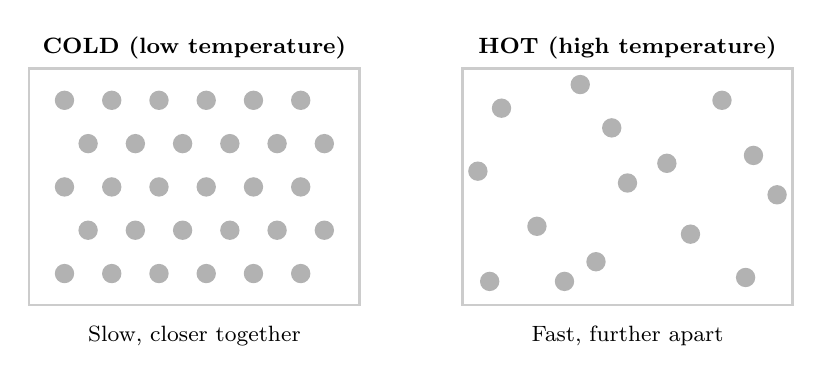
\begin{tikzpicture}[scale=1.0, font=\small]
  % Cold box
  \draw[gray!40, line width=1pt] (0,0) rectangle (4.2,3.0);
  \node[above, font=\footnotesize\bfseries] at (2.1,3.0) {COLD (low temperature)};
  \foreach \x/\y in {
    0.45/0.4,  1.05/0.4,  1.65/0.4,  2.25/0.4,  2.85/0.4,  3.45/0.4,
    0.75/0.95, 1.35/0.95, 1.95/0.95, 2.55/0.95, 3.15/0.95, 3.75/0.95,
    0.45/1.5,  1.05/1.5,  1.65/1.5,  2.25/1.5,  2.85/1.5,  3.45/1.5,
    0.75/2.05, 1.35/2.05, 1.95/2.05, 2.55/2.05, 3.15/2.05, 3.75/2.05,
    0.45/2.6,  1.05/2.6,  1.65/2.6,  2.25/2.6,  2.85/2.6,  3.45/2.6}
    \fill[gray!60] (\x,\y) circle (3.5pt);
  \node[below, font=\footnotesize] at (2.1,-0.15) {Slow, closer together};

  % Hot box
  \draw[gray!40, line width=1pt] (5.5,0) rectangle (9.7,3.0);
  \node[above, font=\footnotesize\bfseries] at (7.6,3.0) {HOT (high temperature)};
  \foreach \x/\y in {
    5.85/0.3,  7.2/0.55,  9.1/0.35,  6.45/1.0,
    8.4/0.9,   9.5/1.4,   5.7/1.7,   7.6/1.55,
    9.2/1.9,   6.0/2.5,   7.4/2.25,  8.8/2.6,
    6.8/0.3,   8.1/1.8,   7.0/2.8}
    \fill[gray!60] (\x,\y) circle (3.5pt);
  \node[below, font=\footnotesize] at (7.6,-0.15) {Fast, further apart};
\end{tikzpicture}
\end{center}

\medskip
\textbf{Label the boxes below:} write ``hot'' or ``cold'' and ``faster'' or ``slower'' under each.

\begin{center}
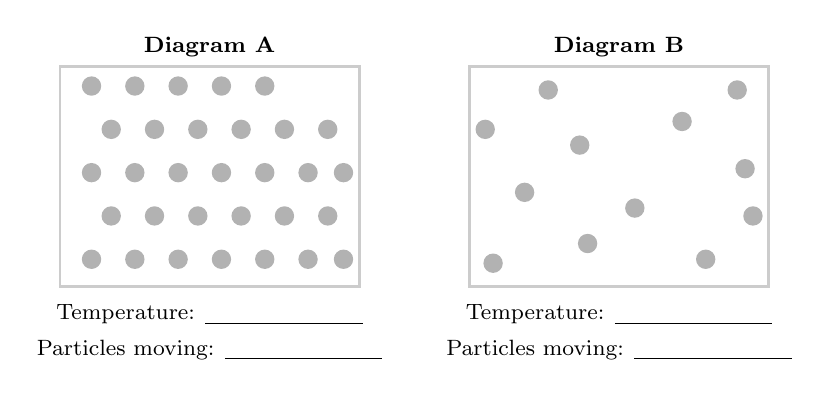
\begin{tikzpicture}[scale=1.0, font=\small]
  % Diagram A — dense (cold)
  \draw[gray!40, line width=1pt] (0,0) rectangle (3.8,2.8);
  \node[above, font=\footnotesize\bfseries] at (1.9,2.8) {Diagram A};
  \foreach \x/\y in {
    0.4/0.35, 0.95/0.35, 1.5/0.35, 2.05/0.35, 2.6/0.35, 3.15/0.35, 3.6/0.35,
    0.65/0.9, 1.2/0.9,  1.75/0.9, 2.3/0.9,  2.85/0.9, 3.4/0.9,
    0.4/1.45, 0.95/1.45, 1.5/1.45, 2.05/1.45, 2.6/1.45, 3.15/1.45, 3.6/1.45,
    0.65/2.0, 1.2/2.0,  1.75/2.0, 2.3/2.0,  2.85/2.0, 3.4/2.0,
    0.4/2.55, 0.95/2.55, 1.5/2.55, 2.05/2.55, 2.6/2.55}
    \fill[gray!60] (\x,\y) circle (3.5pt);
  \node[below, font=\footnotesize] at (1.9,-0.1) {Temperature: \blank{2cm}};
  \node[below, font=\footnotesize] at (1.9,-0.55) {Particles moving: \blank{2cm}};

  % Diagram B — sparse (hot)
  \draw[gray!40, line width=1pt] (5.2,0) rectangle (9.0,2.8);
  \node[above, font=\footnotesize\bfseries] at (7.1,2.8) {Diagram B};
  \foreach \x/\y in {
    5.5/0.3,  6.7/0.55, 8.2/0.35, 8.8/0.9,
    5.9/1.2,  7.3/1.0,  8.7/1.5,
    5.4/2.0,  6.6/1.8,  7.9/2.1,  8.6/2.5,
    6.2/2.5}
    \fill[gray!60] (\x,\y) circle (3.5pt);
  \node[below, font=\footnotesize] at (7.1,-0.1) {Temperature: \blank{2cm}};
  \node[below, font=\footnotesize] at (7.1,-0.55) {Particles moving: \blank{2cm}};
\end{tikzpicture}
\end{center}

\begin{tcolorbox}[misconc]
\textit{``A particle is just a tiny piece of the material --- like a tiny piece of steel.''}

\medskip
This is one of the most common misunderstandings in this unit. A particle in the particle model is \textbf{not} a miniature version of the material. Particles are discrete units with \textbf{empty space between them} --- that space is real, and it is what allows matter to expand and contract. If particles were stuck together with no space, nothing could ever change size with temperature. The space between particles is as important as the particles themselves.
\end{tcolorbox}

\medskip
\textbf{Summarising the particle model:}

\begin{tabularx}{\linewidth}{|X|X|}
\hline
\rowcolor{accentlight}
\textbf{What the model says} & \textbf{Fill in the blank} \\
\hline
All matter is made of & \blank{4cm} \\[6pt]
\hline
Particles have \blank{2.5cm} between them & space \\[6pt]
\hline
Particles are always & \blank{4cm} \\[6pt]
\hline
Heating makes particles move & \blank{2cm} and spread \blank{2cm} \\[6pt]
\hline
Cooling makes particles move & \blank{2cm} and come \blank{2cm} \\[6pt]
\hline
\end{tabularx}

\begin{tcolorbox}[retrieval]
\begin{enumerate}
  \item Name two things the particle model says are always true about particles, no matter what the temperature is.
  \answerline\answerline

  \item What does temperature actually measure, according to the particle model?
  \answerline

  \item What happens to the space between particles when matter is heated?
  \answerline

  \item A student heats a metal rod. Based on the particle model, explain what is happening to the particles inside the rod.
  \answerline\answerline

  \item $\bigstar\bigstar$ A classmate says: ``The particle model is wrong because you can't see particles --- so how do we know they're real?'' How would you respond? Use at least one piece of evidence or reasoning to support the particle model.
  \answerline\answerline\answerline
\end{enumerate}
\end{tcolorbox}

\selfcheck

\smallskip
\noindent\textit{\textbf{Now --- go to the workbook.} You can now answer \textbf{4 questions} in the workbook. Close your notes and go answer them.}

\clearpage

% ============================================================
\section{Section 2: States of Matter and Phase Changes}
% ============================================================

\begin{tcolorbox}[learningtarget]
\textbf{Learning target:} I can describe the particle arrangement and movement in solids, liquids, and gases, name the six phase changes, and explain why mass is conserved during a phase change even when volume changes.
\end{tcolorbox}

\subsection{Vocabulary}

\begin{tabularx}{\linewidth}{|l|X|X|}
\hline
\rowcolor{accentlight}
\textbf{Term} & \textbf{Definition in your own words} & \textbf{One example} \\
\hline
Solid & & \\[14pt]
\hline
Liquid & & \\[14pt]
\hline
Gas & & \\[14pt]
\hline
Phase change & & \\[14pt]
\hline
Melting & & \\[14pt]
\hline
Freezing & & \\[14pt]
\hline
Evaporation & & \\[14pt]
\hline
Condensation & & \\[14pt]
\hline
\end{tabularx}

\subsection{Notes}

\textbf{The three states of matter}

The particle model explains the three states of matter by describing how particles are arranged and how fast they move.

\begin{center}
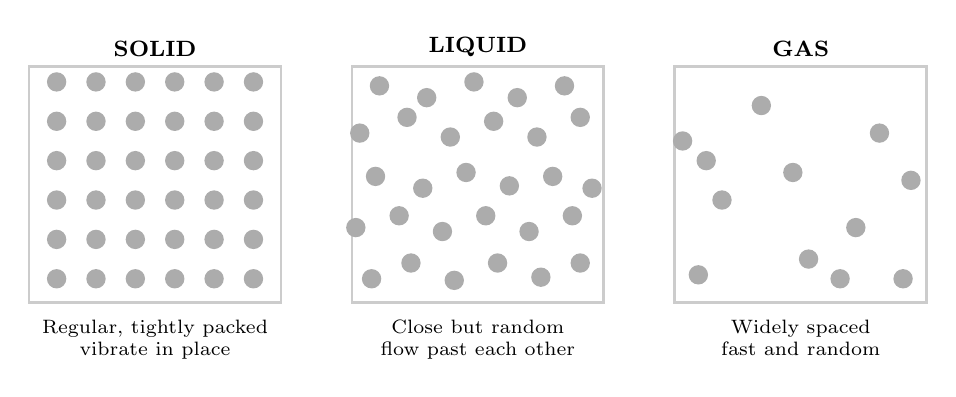
\begin{tikzpicture}[scale=1.0, font=\small]
  % SOLID — regular grid
  \draw[gray!40, line width=1pt] (0,0) rectangle (3.2,3.0);
  \node[above, font=\footnotesize\bfseries] at (1.6,3.0) {SOLID};
  \foreach \x in {0.35, 0.85, 1.35, 1.85, 2.35, 2.85}
    \foreach \y in {0.3, 0.8, 1.3, 1.8, 2.3, 2.8}
      \fill[gray!65] (\x,\y) circle (3.5pt);
  \node[below, font=\scriptsize, align=center] at (1.6,-0.1) {Regular, tightly packed\\vibrate in place};

  % LIQUID — random, close
  \draw[gray!40, line width=1pt] (4.1,0) rectangle (7.3,3.0);
  \node[above, font=\footnotesize\bfseries] at (5.7,3.0) {LIQUID};
  \foreach \x/\y in {
    4.35/0.3,  4.85/0.5,  5.4/0.28, 5.95/0.5,  6.5/0.32, 7.0/0.5,
    4.15/0.95, 4.7/1.1,   5.25/0.9, 5.8/1.1,   6.35/0.9, 6.9/1.1,
    4.4/1.6,   5.0/1.45,  5.55/1.65,6.1/1.48,  6.65/1.6, 7.15/1.45,
    4.2/2.15,  4.8/2.35,  5.35/2.1, 5.9/2.3,   6.45/2.1, 7.0/2.35,
    4.45/2.75, 5.05/2.6,  5.65/2.8, 6.2/2.6,   6.8/2.75}
    \fill[gray!65] (\x,\y) circle (3.5pt);
  \node[below, font=\scriptsize, align=center] at (5.7,-0.1) {Close but random\\flow past each other};

  % GAS — sparse, scattered
  \draw[gray!40, line width=1pt] (8.2,0) rectangle (11.4,3.0);
  \node[above, font=\footnotesize\bfseries] at (9.8,3.0) {GAS};
  \foreach \x/\y in {
    8.5/0.35,  9.9/0.55,  11.1/0.3,
    8.8/1.3,   10.5/0.95, 11.2/1.55,
    8.3/2.05,  9.3/2.5,   10.8/2.15,
    9.7/1.65,  10.3/0.3,  8.6/1.8}
    \fill[gray!65] (\x,\y) circle (3.5pt);
  \node[below, font=\scriptsize, align=center] at (9.8,-0.1) {Widely spaced\\fast and random};
\end{tikzpicture}
\end{center}

\medskip
\textbf{Solid:}
\begin{itemize}[noitemsep, topsep=2pt]
  \item Particles are packed \blank{2cm} together in a regular arrangement
  \item Particles \blank{3cm} (vibrate) but do not move past each other
  \item The shape is \blank{2cm} --- solids hold their shape without a container
  \item The volume is \blank{2cm}
\end{itemize}

\medskip
\textbf{Liquid:}
\begin{itemize}[noitemsep, topsep=2pt]
  \item Particles are \blank{2cm} together but NOT in a fixed arrangement
  \item Particles can slide \blank{2cm} each other --- they flow
  \item The shape is \blank{2cm} --- liquids take the shape of their container
  \item The volume is \blank{2cm} (a liquid doesn't compress easily)
\end{itemize}

\medskip
\textbf{Gas:}
\begin{itemize}[noitemsep, topsep=2pt]
  \item Particles are \blank{2cm} apart --- they fill all available space
  \item Particles move \blank{2cm} and in random directions
  \item The shape is \blank{2cm} --- gases fill their container completely
  \item The volume is \blank{2cm} --- gases can be compressed
\end{itemize}

\medskip
\textbf{Comparison table --- fill in the blanks:}

\begin{tabularx}{\linewidth}{|X|X|X|X|}
\hline
\rowcolor{accentlight}
\textbf{Property} & \textbf{Solid} & \textbf{Liquid} & \textbf{Gas} \\
\hline
Particle spacing & \blank{1.8cm} & close & \blank{1.8cm} \\[6pt]
\hline
Particle movement & vibrate in place & \blank{2cm} past each other & fast and random \\[6pt]
\hline
Fixed shape? & \blank{1.5cm} & No & No \\[6pt]
\hline
Fixed volume? & Yes & \blank{1.5cm} & \blank{1.5cm} \\[6pt]
\hline
\end{tabularx}

\medskip
\textbf{Phase changes --- moving between states}

A \textbf{phase change} happens when matter changes from one state to another. The temperature changes, so the speed of particle movement changes --- enough to change how particles are arranged.

\medskip
\textbf{The six phase changes:}

\begin{tabularx}{\linewidth}{|X|X|X|}
\hline
\rowcolor{accentlight}
\textbf{Change} & \textbf{Direction} & \textbf{Name} \\
\hline
Solid $\rightarrow$ Liquid & Heating & \blank{3.5cm} \\[4pt]
\hline
Liquid $\rightarrow$ Solid & Cooling & \blank{3.5cm} \\[4pt]
\hline
Liquid $\rightarrow$ Gas & Heating & \blank{3.5cm} \\[4pt]
\hline
Gas $\rightarrow$ Liquid & Cooling & \blank{3.5cm} \\[4pt]
\hline
Solid $\rightarrow$ Gas & Heating (rapid) & Sublimation \\[4pt]
\hline
Gas $\rightarrow$ Solid & Cooling (rapid) & Deposition \\[4pt]
\hline
\end{tabularx}

\medskip
\textbf{Phase change diagram --- circle the changes that involve HEATING; box the changes that involve COOLING:}

\begin{center}
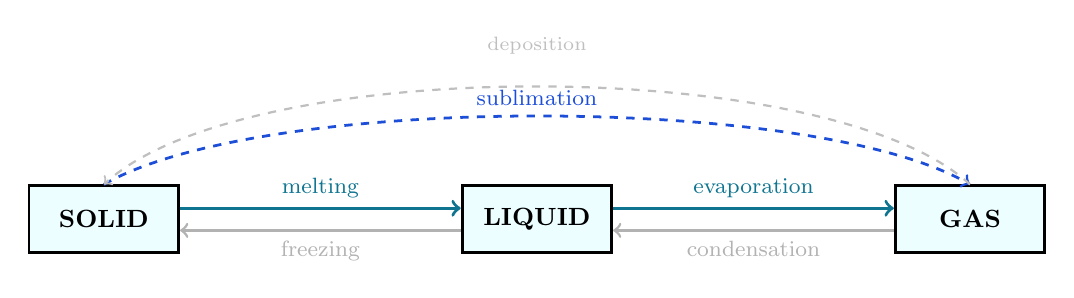
\begin{tikzpicture}[scale=1.0, font=\small]
  \node[draw, line width=1pt, fill=accentlight, minimum width=1.9cm, minimum height=0.85cm,
        font=\small\bfseries] (S) at (0,0) {SOLID};
  \node[draw, line width=1pt, fill=accentlight, minimum width=1.9cm, minimum height=0.85cm,
        font=\small\bfseries] (L) at (5.5,0) {LIQUID};
  \node[draw, line width=1pt, fill=accentlight, minimum width=1.9cm, minimum height=0.85cm,
        font=\small\bfseries] (G) at (11.0,0) {GAS};

  % Solid <-> Liquid
  \draw[->, accent, line width=1.2pt] ([yshift= 4pt]S.east) -- node[above,font=\footnotesize]{melting} ([yshift= 4pt]L.west);
  \draw[->, gray!60, line width=1.0pt] ([yshift=-4pt]L.west) -- node[below,font=\footnotesize]{freezing} ([yshift=-4pt]S.east);

  % Liquid <-> Gas
  \draw[->, accent, line width=1.2pt] ([yshift= 4pt]L.east) -- node[above,font=\footnotesize]{evaporation} ([yshift= 4pt]G.west);
  \draw[->, gray!60, line width=1.0pt] ([yshift=-4pt]G.west) -- node[below,font=\footnotesize]{condensation} ([yshift=-4pt]L.east);

  % Sublimation / deposition (arc above)
  \draw[->, dblue, dashed, line width=1pt]
    (S.north) .. controls (2.0,1.6) and (9.0,1.6) .. (G.north)
    node[midway, above, font=\footnotesize] {sublimation};
  \draw[->, gray!50, dashed, line width=0.8pt]
    (G.north) .. controls (9.2,2.1) and (1.8,2.1) .. (S.north)
    node[midway, above, font=\scriptsize, yshift=8pt] {deposition};
\end{tikzpicture}
\end{center}

\medskip
\textbf{The experimental logic of phase changes:}

Scientists who study phase changes control one variable at a time. To test how temperature affects the phase change of water, you would:
\begin{itemize}[noitemsep, topsep=2pt]
  \item Keep the same \blank{3cm} of water each time
  \item Change only the \blank{3cm} (or the heat source)
  \item Observe the temperature at which the \blank{3cm} happens
\end{itemize}

\medskip
\textbf{CRITICAL IDEA --- Mass is conserved during a phase change:}

When matter changes state, \blank{2cm} is conserved. Only the \blank{2.5cm} and \blank{2.5cm} of the particles change.

\medskip
100\,g of ice $\rightarrow$ melts $\rightarrow$ still \blank{1.5cm}\,g of liquid water

100\,g of liquid water $\rightarrow$ evaporates $\rightarrow$ still \blank{1.5cm}\,g of water vapour

\medskip
The mass does NOT change. Volume, however, \blank{2cm} change during a phase change.

\begin{tcolorbox}[misconc]
\textit{``When ice melts, some of the mass disappears --- that's why there's less water.''}

\medskip
Mass is \textbf{never} created or destroyed during a phase change. The ice and the puddle of water weigh exactly the same. What changes is the \textbf{arrangement} of particles and the \textbf{volume} they take up --- not the number of particles or their mass. If water seems to ``disappear'' when it evaporates, it has not vanished --- it has become water vapour in the air, still carrying the same mass. Conservation of mass is one of the most fundamental laws in science.
\end{tcolorbox}

\begin{tcolorbox}[connection]
\small\textit{Think about a time you saw a phase change in your everyday life. Describe what you saw and name the phase change. Use the particle model to explain what was happening to the particles.}
\answerline\answerline\answerline
\end{tcolorbox}

\begin{tcolorbox}[retrieval]
\begin{enumerate}
  \item Describe the particle arrangement in a solid versus a gas. Use the words ``spacing'' and ``movement'' in your answer.
  \answerline\answerline

  \item Name the phase change that occurs when: (a) liquid water becomes ice, and (b) liquid water becomes water vapour.

  (a) \blank{4.5cm} \qquad (b) \blank{4.5cm}

  \item A student heats 50\,g of ice until it is completely melted. What is the mass of the liquid water?

  \blank{3cm}

  Explain why, using the particle model.
  \answerline

  \item Why does a gas fill the entire container it is placed in, while a solid keeps its own shape?
  \answerline\answerline

  \item $\bigstar\bigstar$ A student claims that boiling water loses mass because ``the steam floats away.'' Write a response that corrects this using the conservation of mass and the particle model. What would you need to measure to prove the student wrong?
  \answerline\answerline\answerline
\end{enumerate}
\end{tcolorbox}

\selfcheck

\smallskip
\noindent\textit{\textbf{Now --- go to the workbook.} You can now answer \textbf{4 questions} in the workbook. Close your notes and go answer them.}

\clearpage

% ============================================================
\section{Section 3: Thermometers and Temperature}
% ============================================================

\begin{tcolorbox}[learningtarget]
\textbf{Learning target:} I can explain how a thermometer works using the particle model, read the Celsius scale, and identify key reference points and safety practices.
\end{tcolorbox}

\subsection{Vocabulary}

\begin{tabularx}{\linewidth}{|l|X|X|}
\hline
\rowcolor{accentlight}
\textbf{Term} & \textbf{Definition in your own words} & \textbf{One example} \\
\hline
Celsius scale & & \\[16pt]
\hline
Reference point & & \\[16pt]
\hline
Thermal expansion & & \\[16pt]
\hline
Calibration & & \\[16pt]
\hline
\end{tabularx}

\subsection{Notes}

\textbf{The Celsius scale}

Temperature is measured in degrees Celsius (\dgr{}C) in science and in everyday life in Canada.

The Celsius scale uses two reference points based on water:

\begin{tabularx}{\linewidth}{|X|X|}
\hline
\rowcolor{accentlight}
\textbf{Reference point} & \textbf{Temperature} \\
\hline
Water \blank{3cm} (liquid $\rightarrow$ solid) & 0\dgr{}C \\[4pt]
\hline
Water \blank{3cm} (liquid $\rightarrow$ gas) & 100\dgr{}C \\[4pt]
\hline
Normal human body temperature & $\approx$37\dgr{}C \\[4pt]
\hline
Room temperature (comfortable) & $\approx$20--22\dgr{}C \\[4pt]
\hline
A cold winter day in Alberta & $\approx -$20\dgr{}C \\[4pt]
\hline
\end{tabularx}

\medskip
These reference points were chosen because they are \blank{3cm} (they always happen at the same temperature, at standard conditions) and easy to reproduce in any lab.

\medskip
\textbf{How a thermometer works}

A traditional liquid thermometer works because of the same particle behaviour you just studied:

\begin{enumerate}
  \item The thermometer contains a liquid (often coloured alcohol) sealed in a glass tube.
  \item When temperature \blank{2.5cm}, the liquid particles move faster and spread further apart. The liquid \blank{2.5cm} and rises up the tube.
  \item When temperature \blank{2.5cm}, the liquid particles slow down and come closer together. The liquid \blank{2.5cm} and falls down the tube.
  \item A scale on the glass shows what temperature the liquid level matches.
\end{enumerate}

The thermometer works because the \blank{3cm} of the liquid changes predictably with temperature.

\medskip
\textbf{Thermometer at two temperatures:}

\begin{center}
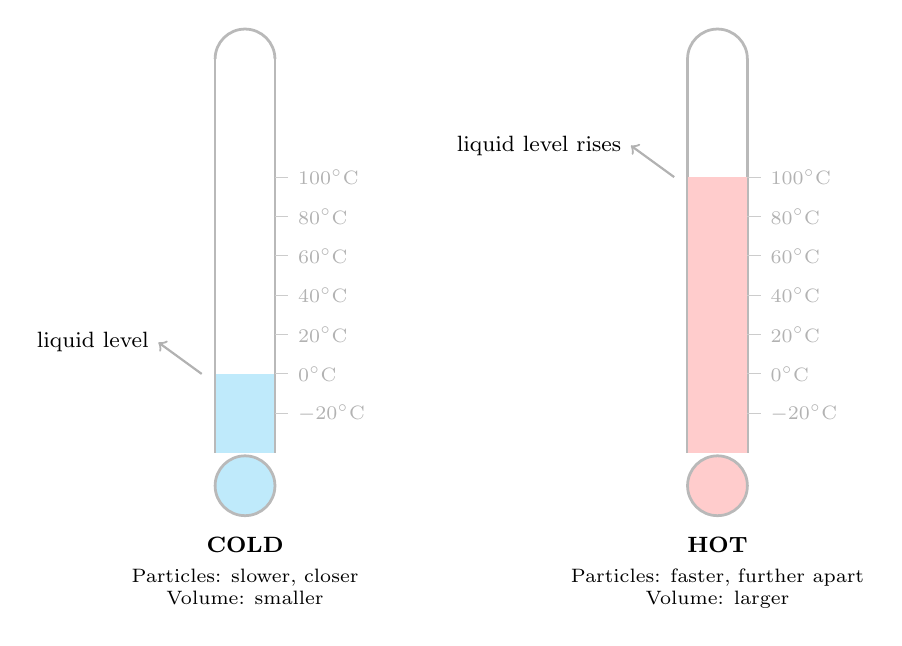
\begin{tikzpicture}[scale=1.0, font=\small]

  % ---- COLD thermometer (liquid at 0 C) ----
  % Bulb
  \fill[cyan!25] (1.0,-0.42) circle (0.38cm);
  \draw[gray!55, line width=1pt] (1.0,-0.42) circle (0.38cm);
  % Tube outline
  \draw[gray!55, line width=1pt] (0.62,0) -- (0.62,5.0);
  \draw[gray!55, line width=1pt] (1.38,0) -- (1.38,5.0);
  \draw[gray!55, line width=1pt] (0.62,5.0) arc(180:0:0.38cm);
  % Liquid fill (0 C = y=1.0 on our scale)
  \fill[cyan!25] (0.63,0) rectangle (1.37,1.0);
  % Tick marks + labels
  \draw[gray!40] (1.38,0.5)  -- (1.55,0.5);  \node[right,font=\scriptsize,gray!60] at (1.55,0.5)  {$-20$\dgr{}C};
  \draw[gray!40] (1.38,1.0)  -- (1.55,1.0);  \node[right,font=\scriptsize,gray!60] at (1.55,1.0)  {0\dgr{}C};
  \draw[gray!40] (1.38,1.5)  -- (1.55,1.5);  \node[right,font=\scriptsize,gray!60] at (1.55,1.5)  {20\dgr{}C};
  \draw[gray!40] (1.38,2.0)  -- (1.55,2.0);  \node[right,font=\scriptsize,gray!60] at (1.55,2.0)  {40\dgr{}C};
  \draw[gray!40] (1.38,2.5)  -- (1.55,2.5);  \node[right,font=\scriptsize,gray!60] at (1.55,2.5)  {60\dgr{}C};
  \draw[gray!40] (1.38,3.0)  -- (1.55,3.0);  \node[right,font=\scriptsize,gray!60] at (1.55,3.0)  {80\dgr{}C};
  \draw[gray!40] (1.38,3.5)  -- (1.55,3.5);  \node[right,font=\scriptsize,gray!60] at (1.55,3.5)  {100\dgr{}C};
  % Level arrow
  \draw[->, gray!60, line width=0.8pt] (0.45,1.0) -- (-0.1,1.4);
  \node[left,font=\footnotesize] at (-0.1,1.4) {liquid level};
  % Labels below
  \node[below,font=\footnotesize\bfseries] at (1.0,-0.95) {COLD};
  \node[below,font=\scriptsize,align=center] at (1.0,-1.35) {Particles: slower, closer\\Volume: smaller};

  % ---- HOT thermometer (liquid at 100 C) ----
  \fill[red!20] (7.0,-0.42) circle (0.38cm);
  \draw[gray!55, line width=1pt] (7.0,-0.42) circle (0.38cm);
  \draw[gray!55, line width=1pt] (6.62,0) -- (6.62,5.0);
  \draw[gray!55, line width=1pt] (7.38,0) -- (7.38,5.0);
  \draw[gray!55, line width=1pt] (6.62,5.0) arc(180:0:0.38cm);
  % Liquid fill (100 C = y=3.5)
  \fill[red!20] (6.63,0) rectangle (7.37,3.5);
  % Tick marks + labels
  \draw[gray!40] (7.38,0.5)  -- (7.55,0.5);  \node[right,font=\scriptsize,gray!60] at (7.55,0.5)  {$-20$\dgr{}C};
  \draw[gray!40] (7.38,1.0)  -- (7.55,1.0);  \node[right,font=\scriptsize,gray!60] at (7.55,1.0)  {0\dgr{}C};
  \draw[gray!40] (7.38,1.5)  -- (7.55,1.5);  \node[right,font=\scriptsize,gray!60] at (7.55,1.5)  {20\dgr{}C};
  \draw[gray!40] (7.38,2.0)  -- (7.55,2.0);  \node[right,font=\scriptsize,gray!60] at (7.55,2.0)  {40\dgr{}C};
  \draw[gray!40] (7.38,2.5)  -- (7.55,2.5);  \node[right,font=\scriptsize,gray!60] at (7.55,2.5)  {60\dgr{}C};
  \draw[gray!40] (7.38,3.0)  -- (7.55,3.0);  \node[right,font=\scriptsize,gray!60] at (7.55,3.0)  {80\dgr{}C};
  \draw[gray!40] (7.38,3.5)  -- (7.55,3.5);  \node[right,font=\scriptsize,gray!60] at (7.55,3.5)  {100\dgr{}C};
  % Level arrow
  \draw[->, gray!60, line width=0.8pt] (6.45,3.5) -- (5.9,3.9);
  \node[left,font=\footnotesize] at (5.9,3.9) {liquid level rises};
  % Labels below
  \node[below,font=\footnotesize\bfseries] at (7.0,-0.95) {HOT};
  \node[below,font=\scriptsize,align=center] at (7.0,-1.35) {Particles: faster, further apart\\Volume: larger};

\end{tikzpicture}
\end{center}

\medskip
\textbf{Safety practices --- thermometers in the lab}

\begin{itemize}[noitemsep, topsep=2pt]
  \item Never \blank{3cm} the thermometer --- hold it gently; it can crack under pressure
  \item Never use a thermometer to \blank{3cm} liquids --- it is not a stirring rod
  \item If a thermometer \blank{3cm}, do not touch the glass or liquid --- notify your teacher
  \item Read the thermometer at \blank{3cm} --- your eye should be level with the liquid surface (parallax error if read from above or below)
  \item Wait for the reading to \blank{3cm} before recording --- the liquid needs time to reach the temperature of the substance
\end{itemize}

\begin{tcolorbox}[connection]
\small\textit{Digital thermometers do not use liquid expansion. They use a tiny electrical sensor that changes resistance with temperature. The reading on the screen is still in Celsius. What do you think stays the same between a liquid thermometer and a digital thermometer, and what is different?}
\answerline\answerline
\end{tcolorbox}

\begin{tcolorbox}[retrieval]
\begin{enumerate}
  \item What are the two reference points on the Celsius scale? Give the temperature for each.
  \answerline

  \item Explain, using the particle model, why the liquid in a thermometer rises when temperature increases.
  \answerline\answerline

  \item A student reads a thermometer from above the liquid level. What kind of error might this cause?
  \answerline

  \item A student uses the thermometer to stir a beaker of hot water. What could go wrong, and why?
  \answerline

  \item $\bigstar\bigstar$ The Celsius scale is described as ``calibrated to water.'' What does this mean, and why does using water as the reference make the scale useful for both everyday life and science experiments involving living things?
  \answerline\answerline\answerline
\end{enumerate}
\end{tcolorbox}

\selfcheck

\smallskip
\noindent\textit{\textbf{Now --- go to the workbook.} You can now answer \textbf{3 questions} in the workbook. Close your notes and go answer them.}

\clearpage

% ============================================================
\section{Section 4: Expansion, Contraction, and the Water Anomaly}
% ============================================================

\begin{tcolorbox}[learningtarget]
\textbf{Learning target:} I can explain why most materials expand when heated and contract when cooled, describe real-world applications, explain why water is an exception, and use the particle model to explain why ice floats.
\end{tcolorbox}

\subsection{Vocabulary}

\begin{tabularx}{\linewidth}{|l|X|X|}
\hline
\rowcolor{accentlight}
\textbf{Term} & \textbf{Definition in your own words} & \textbf{One example} \\
\hline
Expansion & & \\[16pt]
\hline
Contraction & & \\[16pt]
\hline
Density & & \\[16pt]
\hline
Anomaly & & \\[16pt]
\hline
Expansion joint & & \\[16pt]
\hline
\end{tabularx}

\subsection{Notes}

\textbf{The general rule: expansion and contraction}

\begin{itemize}[noitemsep, topsep=2pt]
  \item When a material is \blank{2.5cm}, its particles move faster and spread further apart. The material takes up more space --- it \blank{2.5cm}.
  \item When a material is \blank{2.5cm}, its particles slow down and move closer together. The material takes up less space --- it \blank{2.5cm}.
\end{itemize}

This applies to solids, liquids, and gases --- though gases expand and contract far more dramatically.

\medskip
\textbf{Real-world applications:}

Engineers must account for expansion and contraction in design. Materials fixed rigidly in place that cannot expand will \blank{3cm}, crack, or buckle.

\medskip
\textbf{Expansion joints in bridges and roads:}

Long bridges are not one continuous piece. Engineers leave small \blank{3cm} between sections --- called expansion joints.

\begin{center}
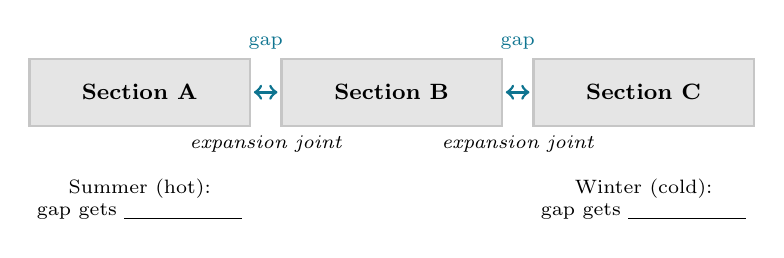
\begin{tikzpicture}[scale=1.0, font=\small]
  % Three bridge sections
  \fill[gray!20] (0,0) rectangle (2.8,0.85);
  \fill[gray!20] (3.2,0) rectangle (6.0,0.85);
  \fill[gray!20] (6.4,0) rectangle (9.2,0.85);
  \draw[gray!45, line width=0.8pt] (0,0) rectangle (2.8,0.85);
  \draw[gray!45, line width=0.8pt] (3.2,0) rectangle (6.0,0.85);
  \draw[gray!45, line width=0.8pt] (6.4,0) rectangle (9.2,0.85);

  \node[font=\footnotesize\bfseries] at (1.4,0.425) {Section A};
  \node[font=\footnotesize\bfseries] at (4.6,0.425) {Section B};
  \node[font=\footnotesize\bfseries] at (7.8,0.425) {Section C};

  % Gap markers
  \draw[<->, accent, line width=1pt] (2.85,0.425) -- (3.15,0.425);
  \draw[<->, accent, line width=1pt] (6.05,0.425) -- (6.35,0.425);
  \node[above,font=\scriptsize\color{accent}] at (3.0,0.85) {gap};
  \node[above,font=\scriptsize\color{accent}] at (6.2,0.85) {gap};
  \node[below,font=\scriptsize\itshape] at (3.0,0) {expansion joint};
  \node[below,font=\scriptsize\itshape] at (6.2,0) {expansion joint};

  % Summer / winter labels
  \node[below,font=\scriptsize,align=center] at (1.4,-0.55) {Summer (hot):\\gap gets \blank{1.5cm}};
  \node[below,font=\scriptsize,align=center] at (7.8,-0.55) {Winter (cold):\\gap gets \blank{1.5cm}};
\end{tikzpicture}
\end{center}

Without expansion joints, the force of expansion would \blank{3cm} the bridge.

\medskip
\textbf{Gaps in railway tracks:} Traditional rail sections also leave small gaps for the same reason. Modern continuous welded rail is pre-stressed to account for \blank{3cm}.

\medskip
\textbf{Power lines:} Electrical lines hang lower in \blank{2.5cm} (heat causes sagging) and are pulled tighter in \blank{2.5cm} (cold causes contraction).

\begin{tcolorbox}[connection]
\small\textit{Look at the road or a bridge near your school. Why would a road in Alberta need larger expansion joints than a road built in a tropical region with stable temperatures year-round?}
\answerline\answerline
\end{tcolorbox}

\medskip
\textbf{The water anomaly --- when the general rule breaks}

For almost every material, the solid is \blank{3cm} than the liquid (tightly packed = smaller volume for same mass = higher density).

Water breaks this rule. This is called the \textbf{water anomaly}. When water freezes:
\begin{itemize}[noitemsep, topsep=2pt]
  \item Most liquids become more \blank{2.5cm} when they solidify
  \item Water becomes \blank{2.5cm} dense when it freezes
\end{itemize}

Ice takes up \blank{2.5cm} space than the same mass of liquid water. Ice is less dense than liquid water. This is why ice \blank{2cm}.

\medskip
\textbf{Why water is different --- the particle model explanation:}

When water freezes, particles lock into a crystal structure with a \blank{3cm} arrangement that actually pushes particles \textit{further apart} --- creating more space, not less.

\begin{center}
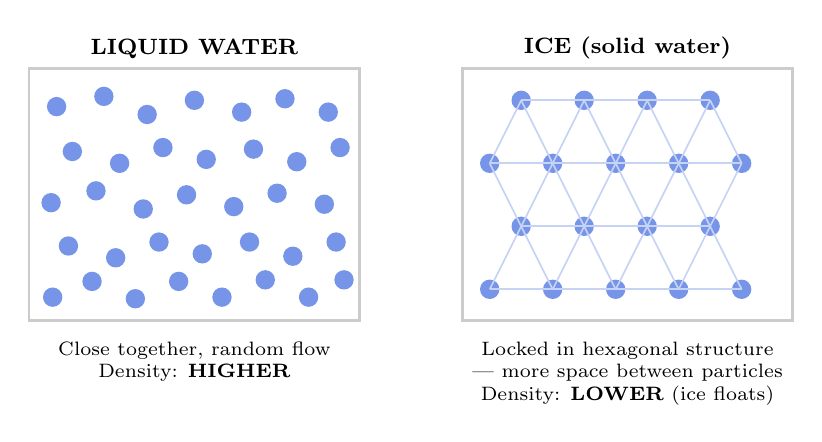
\begin{tikzpicture}[scale=1.0, font=\small]
  % Liquid water — random, closely packed
  \draw[gray!40, line width=1pt] (0,0) rectangle (4.2,3.2);
  \node[above,font=\footnotesize\bfseries] at (2.1,3.2) {LIQUID WATER};
  \foreach \x/\y in {
    0.3/0.3,   0.8/0.5,   1.35/0.28, 1.9/0.5,   2.45/0.3,  3.0/0.52,  3.55/0.3,  4.0/0.52,
    0.5/0.95,  1.1/0.8,   1.65/1.0,  2.2/0.85,  2.8/1.0,   3.35/0.82, 3.9/1.0,
    0.28/1.5,  0.85/1.65, 1.45/1.42, 2.0/1.6,   2.6/1.45,  3.15/1.62, 3.75/1.48,
    0.55/2.15, 1.15/2.0,  1.7/2.2,   2.25/2.05, 2.85/2.18, 3.4/2.02,  3.95/2.2,
    0.35/2.72, 0.95/2.85, 1.5/2.62,  2.1/2.8,   2.7/2.65,  3.25/2.82, 3.8/2.65}
    \fill[dblue!60] (\x,\y) circle (3.5pt);
  \node[below,font=\scriptsize,align=center] at (2.1,-0.15) {Close together, random flow\\Density: \textbf{HIGHER}};

  % Ice — hexagonal offset, more space
  \draw[gray!40, line width=1pt] (5.5,0) rectangle (9.7,3.2);
  \node[above,font=\footnotesize\bfseries] at (7.6,3.2) {ICE (solid water)};
  % Row 1 (y=0.4): 5 particles at x = 5.85, 6.65, 7.45, 8.25, 9.05
  % Row 2 (y=1.2): 4 particles, offset — x = 6.25, 7.05, 7.85, 8.65
  % Row 3 (y=2.0): 5 particles same as row 1
  % Row 4 (y=2.8): 4 particles same as row 2
  \foreach \x/\y in {
    5.85/0.4, 6.65/0.4, 7.45/0.4, 8.25/0.4, 9.05/0.4,
    6.25/1.2, 7.05/1.2, 7.85/1.2, 8.65/1.2,
    5.85/2.0, 6.65/2.0, 7.45/2.0, 8.25/2.0, 9.05/2.0,
    6.25/2.8, 7.05/2.8, 7.85/2.8, 8.65/2.8}
    \fill[dblue!60] (\x,\y) circle (3.5pt);
  % Horizontal bonds within rows
  \foreach \y in {0.4, 2.0} {
    \draw[dblue!25,line width=0.6pt] (5.85,\y)--(6.65,\y);
    \draw[dblue!25,line width=0.6pt] (6.65,\y)--(7.45,\y);
    \draw[dblue!25,line width=0.6pt] (7.45,\y)--(8.25,\y);
    \draw[dblue!25,line width=0.6pt] (8.25,\y)--(9.05,\y);
  }
  \foreach \y in {1.2, 2.8} {
    \draw[dblue!25,line width=0.6pt] (6.25,\y)--(7.05,\y);
    \draw[dblue!25,line width=0.6pt] (7.05,\y)--(7.85,\y);
    \draw[dblue!25,line width=0.6pt] (7.85,\y)--(8.65,\y);
  }
  % Diagonal bonds row1->row2
  \foreach \xs/\xe in {5.85/6.25, 6.65/6.25, 6.65/7.05, 7.45/7.05, 7.45/7.85, 8.25/7.85, 8.25/8.65, 9.05/8.65}
    \draw[dblue!25,line width=0.6pt] (\xs,0.4)--(\xe,1.2);
  % Diagonal bonds row2->row3
  \foreach \xs/\xe in {6.25/5.85, 6.25/6.65, 7.05/6.65, 7.05/7.45, 7.85/7.45, 7.85/8.25, 8.65/8.25, 8.65/9.05}
    \draw[dblue!25,line width=0.6pt] (\xs,1.2)--(\xe,2.0);
  % Diagonal bonds row3->row4
  \foreach \xs/\xe in {5.85/6.25, 6.65/6.25, 6.65/7.05, 7.45/7.05, 7.45/7.85, 8.25/7.85, 8.25/8.65, 9.05/8.65}
    \draw[dblue!25,line width=0.6pt] (\xs,2.0)--(\xe,2.8);

  \node[below,font=\scriptsize,align=center] at (7.6,-0.15) {Locked in hexagonal structure\\--- more space between particles\\Density: \textbf{LOWER} (ice floats)};
\end{tikzpicture}
\end{center}

\begin{tcolorbox}[misconc]
\textit{``Ice is denser than liquid water --- solids are always denser than liquids.''}

\medskip
For most materials, this is true --- but \textbf{water is a major exception}. Ice is \textbf{less} dense than liquid water. This is why ice floats at the surface rather than sinking to the bottom. The reason is the structure water forms when it freezes: a hexagonal crystal lattice that takes up \textbf{more} space than randomly arranged liquid water particles. This is not a small exception --- it has enormous consequences for life on Earth.
\end{tcolorbox}

\medskip
\textbf{Why the water anomaly matters:}

\textbf{Aquatic life in winter:} When a lake cools, ice forms on the \blank{2.5cm} and floats. The liquid water beneath stays at approximately \blank{2cm} --- cold, but not frozen. Fish and other organisms survive in the liquid layer \blank{1.5cm}. If ice sank, lakes could freeze \blank{2cm} to \blank{2cm} and most aquatic life would not survive.

\medskip
\textbf{Infrastructure:} Water that seeps into rock cracks and freezes expands, breaking rock apart --- called freeze-thaw weathering. Engineers designing roads in cold climates must account for this in drainage design.

\begin{tcolorbox}[fnmi]
\small Cree, Den\'e, and M\'etis communities in northern Alberta have observed and documented seasonal freeze-thaw cycles on rivers and lakes for generations. This knowledge includes when ice is thick enough for travel, how ice changes near river currents, and how early melt or late freeze signals broader ecological shifts. This is a form of long-term data collection --- systematic observation across seasons and years --- that aligns with what scientists now measure using sensors and satellite data. Both are ways of tracking the same real patterns.
\end{tcolorbox}

\medskip
\textbf{The water anomaly as a testable prediction:}

Most people would predict ice sinks. The particle model, if incorrectly applied, predicts: solid is denser, so solid sinks. The observation --- ice floats --- \textbf{surprises} that prediction. This is exactly how science works: when a result surprises your prediction, you do not discard the observation. You \textit{revise your model}. The hexagonal crystal structure explanation came \textit{after} scientists observed that ice floats and had to figure out why.

\medskip
\textbf{Summarising expansion, contraction, and the water anomaly:}

\begin{tabularx}{\linewidth}{|X|X|X|}
\hline
\rowcolor{accentlight}
\textbf{Situation} & \textbf{What happens} & \textbf{Why} \\
\hline
Metal rod heated & \blank{3cm} & Particles move faster, spread apart \\[6pt]
\hline
Metal rod cooled & \blank{3cm} & Particles slow down, come closer \\[6pt]
\hline
Water heated (liquid) & expands slightly & Particle spacing increases \\[6pt]
\hline
Water cooled to 0\dgr{}C and frozen & \blank{3cm} (anomaly) & Crystal structure pushes particles \blank{2cm} \\[6pt]
\hline
\end{tabularx}

\begin{tcolorbox}[retrieval]
\begin{enumerate}
  \item What is the general rule for how most materials behave when heated?
  \answerline

  \item What is an expansion joint, and why do bridges need them?
  \answerline\answerline

  \item Ice floats on liquid water. What does this tell you about the density of ice compared to liquid water?
  \answerline

  \item Why can fish survive in an ice-covered lake in winter? Use the words ``density'' and ``layer'' in your answer.
  \answerline\answerline

  \item $\bigstar\bigstar$ A student says: ``The fact that ice floats proves the particle model is wrong, because solids are supposed to be denser.'' Is this a correct critique of the particle model? Explain why the water anomaly does not disprove the model --- and what it actually shows about how science works when observations surprise predictions.
  \answerline\answerline\answerline
\end{enumerate}
\end{tcolorbox}

\selfcheck

\smallskip
\noindent\textit{\textbf{Now --- go to the workbook.} You can now answer \textbf{5 questions} in the workbook. Close your notes and go answer them.}

\clearpage

% ============================================================
\section*{Unit Synthesis --- From Memory}
% ============================================================

\textit{Close your notes. Reconstruct.}

\medskip
For each section, write the single most important idea in one sentence --- from memory, no looking back.

\medskip
\textbf{Section 1 --- The Particle Model}
\answerline

\medskip
\textbf{Section 2 --- States of Matter and Phase Changes}
\answerline

\medskip
\textbf{Section 3 --- Thermometers and Temperature}
\answerline

\medskip
\textbf{Section 4 --- Expansion, Contraction, and the Water Anomaly}
\answerline

\medskip
\textit{Now open your notes and check.}

\medskip\noindent\rule{\linewidth}{0.4pt}\medskip

\textbf{Guiding question for this unit:} How can the particles of matter be influenced by heating or cooling?

Write your answer in 3--5 sentences from memory. Use at least three science vocabulary terms from this unit.

\answerline\answerline\answerline\answerline\answerline

\medskip\noindent\rule{\linewidth}{0.4pt}\medskip

\textbf{Final step --- return to your Pre-Knowledge Check.} Read what you wrote before the unit began.

\medskip
What did you get right? \blank{10cm}

\medskip
What were you wrong about? \blank{9.5cm}

\medskip
What surprised you most? \blank{9.5cm}

\clearpage

% ============================================================
\section*{Self-Assessment Rubric}
% ============================================================

\textit{Rate yourself honestly after the final session. Use this to identify what to review before the unit test.}

\begin{tabularx}{\linewidth}{|X|p{4.5cm}|X|}
\hline
\rowcolor{accentlight}
\textbf{Knowledge cluster} & \textbf{I can explain this without notes} & \textbf{One question I still have} \\
\hline
Particle model: particles have space, always move, speed changes with temperature &
Yes \quad Getting there \quad Not yet & \\[20pt]
\hline
Three states of matter: particle arrangement and movement in solid, liquid, gas &
Yes \quad Getting there \quad Not yet & \\[20pt]
\hline
Phase changes: names, directions, and conservation of mass &
Yes \quad Getting there \quad Not yet & \\[20pt]
\hline
Thermometers: how they work, Celsius scale, reference points, safety &
Yes \quad Getting there \quad Not yet & \\[20pt]
\hline
Expansion and contraction: general rule, real-world applications &
Yes \quad Getting there \quad Not yet & \\[20pt]
\hline
Water anomaly: ice is less dense, floats, why this matters for aquatic life &
Yes \quad Getting there \quad Not yet & \\[20pt]
\hline
\end{tabularx}

\smallskip
\textit{Bring your unanswered questions to class. They will appear on the inquiry project and the unit test.}

\end{document}
